\documentclass[
  captions=tableheading,
  bibliography=totoc, 
  titepage=firstiscover,
]{scrartcl}

\usepackage{blindtext} %neuer input

\usepackage{longtable} % Tabellen über mehrere Seiten

\usepackage[utf8]{inputenc} %neuer input

\usepackage{scrhack}

\usepackage[aux]{rerunfilecheck} %Warnung falls nochmal kompiliert werden muss

\usepackage{fontspec} %Fonteinstellungen

\recalctypearea{}

\usepackage[main=ngerman]{babel} %deutsche Spracheinstellung

\usepackage{ragged2e} %neuer input

\usepackage{amsmath, nccmath}

\usepackage{amssymb} %viele mathe Symbole

\usepackage{mathtools} %Erweiterungen für amsmath


\DeclarePairedDelimiter{\abs}{\lvert}{\rvert}
\DeclarePairedDelimiter{\norm}{\lVert}{\rVert}

\DeclarePairedDelimiter{\bra}{\langle}{\rvert}
\DeclarePairedDelimiter{\ket}{\lvert}{\rangle}

\DeclarePairedDelimiterX{\braket}[2]{\langle}{\rangle}{
#1 \delimsize| #2
}

\NewDocumentCommand \dif {m}
{
\mathinner{\symup{d} #1}
}


\usepackage[
  math-style=ISO,
  bold-style=ISO,
  sans-style=italic,
  nabla=upright,
  partial=upright,
  warnings-off={
    mathtools-colon,
    mathtools-overbracket,
  },
]{unicode-math}

\setmathfont{Latin Modern Math}
\setmathfont{XITS Math}[range={scr, bfscr}]
\setmathfont{XITS Math}[range={cal, bfcal}, StylisticSet=1]


\usepackage[
  locale=DE,
  separate-uncertainty=true,
  per-mode=reciprocal,
  output-decimal-marker={,},
]{siunitx}

\usepackage[autostyle]{csquotes} %richtige Anführungszeichen

\usepackage{xfrac}

\usepackage{float}

\floatplacement{figure}{htbp}

\floatplacement{table}{htbp}

\usepackage[ %floats innerhalb einer section halten
  section,   %floats innerhalb er section halten
  below,     %unterhalb der Section aber auf der selben Seite ist ok
]{placeins}

\usepackage[
  labelfont=bf,
  font=small,
  width=0.9\textwidth,
]{caption}

\usepackage{subcaption} %subfigure, subtable, subref

\usepackage{graphicx}

\usepackage{grffile}

\usepackage{booktabs}

\usepackage{microtype} %Verbesserungen am Schriftbild

\usepackage[
backend=biber,
]{biblatex}

\addbibresource{../lit.bib}

\usepackage[ %Hyperlinks im Dokument
  german,
  unicode,
  pdfusetitle,
  pdfcreator={},
  pdfproducer={},
]{hyperref}

\usepackage{bookmark}

\usepackage[shortcuts]{extdash}

%\usepackage{warpcol}

\usepackage{physics}
\allowdisplaybreaks

\begin{document}
    \title{Physik IV Übungsblatt 10}
    \author{  
    Tobias Rücker\\
    \texorpdfstring{\href{mailto:tobias.ruecker@tu-dortmund.de}{tobias.ruecker@tu-dortmund.de}
    \and}{,} 
    Paul Störbrock\\
    \texorpdfstring{\href{mailto:paul.stoerbrock@tu-dortmund.de}{paul.stoerbrock@tu-dortmund.de}}{}
    }
\maketitle
\center{\Large Abgabegruppe: \textbf{4H}}
\thispagestyle{empty}

\newpage
\tableofcontents
\thispagestyle{empty}
\newpage

\setcounter{page}{1}

\section{Aufgabe 1}

    \begin{figure}[H]
        \centering
        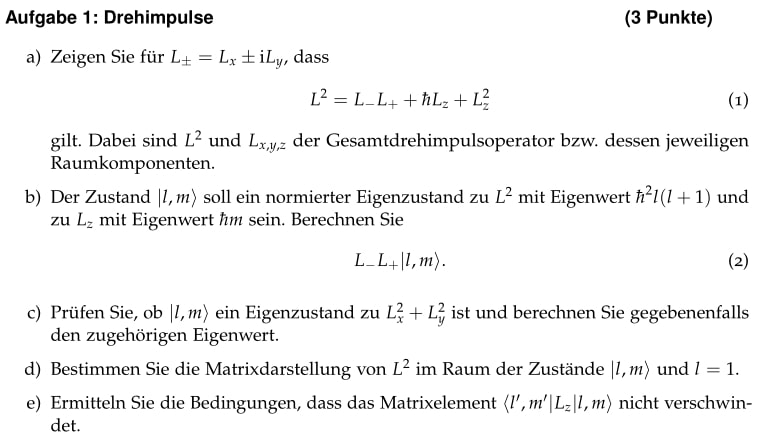
\includegraphics[width=\textwidth]{images/Aufgabe1.jpg}
        \label{fig:1}
    \end{figure}

\subsection{a)}

    \begin{align}
        L_{\pm} &= L_x \pm iL_y\\
        \left[ L_x,L_y \right] &= i\hbar L_z \qquad \Rightarrow \text{Den Kommutator schnappen wir uns aus Übung 7 (Aufg.3b)}\\
        \\
        L_- L_+ &= \left( L_x - iL_y \right)\left( L_x + iL_y \right)\\
        &= L_x^2 + iL_x L_y - iL_y L_x + L_y^2\\
        &= L_x^2 + L_y^2 + i\underbrace{\left( L_x L_y - L_y L_x \right)}_{=\left[L_x,L_y\right]}\\
        &= L_x^2 + L_y^2 \underbrace{+ L_z^2 - L_z^2}_{Nulladdition} + i \left( i\hbar L_z\right)\\
        &= \underbrace{L_x^2 + L_y^2 + L_z^2}_{=L^2} - L_z^2 - \hbar L_z\\
        L_{\pm} &= L^2 - \hbar L_z - L_z^2\\
        \Leftrightarrow L^2 &= L_{\pm} + \hbar L_z + L_z^2
    \end{align}

\subsection{b)}

    \begin{align}
        L^2 \ket{l,m} &= \hbar^2 l(l+1) \ket{l,m}\\
        L_z \ket{l,m} &= \hbar m \ket{l,m}\\
        \\
        L_- L_+ \ket{l,m} &= \left( L^2 - \hbar L_z - L_z^2 \right) \ket{l,m}\\
        &= \left( \hbar^2 l(l+1) - \hbar^2 m - \hbar^2 m^2 \right) \ket{l,m}\\
        &= \hbar^2 \left( l(l+1) \underbrace{- m - m^2}_{=-m(m+1)} \right) \ket{l,m}\\
        &= \hbar^2 \left( l(l+1) -m(m+1) \right) \ket{l,m}
    \end{align}

\subsection{c)}

    \begin{align}
        \left( L_x^2 + L_y^2 \right) \ket{l,m} &= \left( L_- L_+ + \hbar L_z \right) \ket{l,m}\\
        &= \left[ \hbar^2 \left( l(l+1) - m(m+1) \right) + \hbar^2 m  \right] \ket{l,m}\\
        &= \hbar^2 \left( l(l+1) - m(m+1) + m \right) \ket{l,m}\\
        &= \hbar^2 \left( l(l+1) - m^2 -m + m \right) \ket{l,m}\\
        &= \hbar^2 \left( l(l+1) - m^2 \right) \ket{l,m}
    \end{align}

\subsection{d)}

    \begin{align}
        \bra{l',m'} L^2 \ket{l,m} &= \hbar^2 l(l+1) \delta_{mm}'\\
        \bra{l',m'} L^2 \ket{l,m} &= \bra{l',m'} L_- L_+ + \hbar L_z + L_z^2 \ket{l,m'}\\
        &= \bra{l',m'} \hbar^2 l(l+1) \ket{l,m}\\
        &= \hbar^2 l(l+1) \underbrace{\braket{l',m'}{l,m}}_{=\delta_{mm'}\delta_{ll'}}\\
        &= \hbar^2 l(l+1) \delta_{mm'} \delta_{ll'}\\
        &\stackrel{l=1}{=} 2\hbar \delta_{mm'} \delta_{1l'} 
        \intertext{
            \flushleft{Maximal\;}\justifying für $m=l$:
        }
        L_+ \ket{l,l} &=0
        \intertext{
             \flushleft{Minimum:\;}\justifying
        }
        L_- \ket{l,l'} &=0\\
        l(l+1) &= l'(l'+1)\\
        l' &= -l\\
        \Rightarrow &\text{Minimal für $m=-l$.}\\
        m &= -l, ..., l
        \intertext{
            \flushleft{Bei\;}\justifying einem Intervall von $-l \leq m \leq l$ ist die Dimension des Unterraums von $m$ gleich 2l+1, was für $l=1$ eine Dimension von 3 ergibt.
            Daraus folgt die Matrix:
        }
        L^2 &= 2\hbar^2 \begin{pmatrix}
            1 & 0 & 0\\
            0 & 1 & 0\\
            0 & 0 & 1
        \end{pmatrix}
    \end{align}

\subsection{e)}

    \flushleft{Zuerst\;}\justifying lässt sich aus der Beziehung $L_z \ket{l,m} = \hbar m \ket{l,m}$ erkennen, dass $m\neq 0$ sein muss, ansonsten würde das Matrixelement sofort 
    verschwinden. Desweiteren gilt:
    \begin{align}
        \bra{l',m'} L_z \ket{l,m} &= \hbar m \braket{l',m'}{l,m}\\
        &= \hbar m \delta_{mm'} \delta_{ll'} 
    \end{align}
    \flushleft{Aus\;}\justifying der Deltafunktion geht hervor, dass $m=m'=l=l'$ sein muss, da $L_z$ sonst $=0$ sein würde, wodurch das Matrixelement verschwindet. Daraus folgt,
    dass $L_z$ die Bedingungen $m=m'=l=l'\neq 0$ erfüllen muss, damit das Matrixelement erhalten bleibt. 

\section{Aufgabe 2}

    \begin{figure}[H]
        \centering
        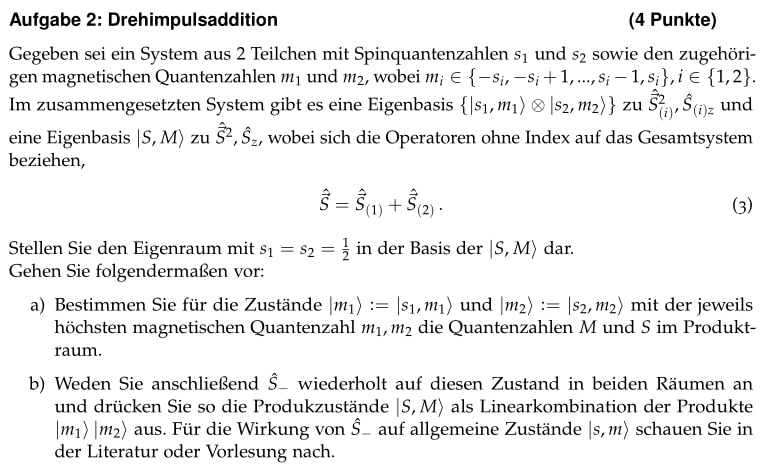
\includegraphics[width=\textwidth]{images/Aufgabe2a.jpg}
        \label{fig:2}
    \end{figure}

    \begin{figure}[H]
        \centering
        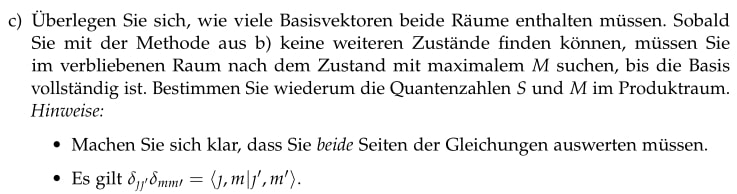
\includegraphics[width=\textwidth]{images/Aufgabe2b.jpg}
        \label{fig:3}
    \end{figure}

\subsection{a)}

\subsection{b)}

\subsection{c)}

\section{Aufgabe 3}

    \begin{figure}[H]
        \centering
        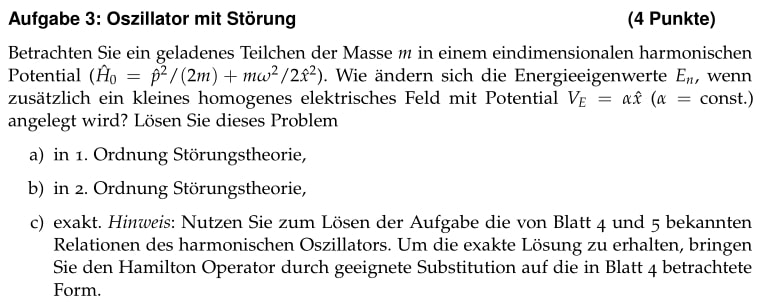
\includegraphics[width=\textwidth]{images/Aufgabe3.jpg}
        \label{fig:4}
    \end{figure}

\subsection{a)}

\subsection{b)}

\subsection{c)}

\section{Aufgabe 4}

    \begin{figure}[H]
        \centering
        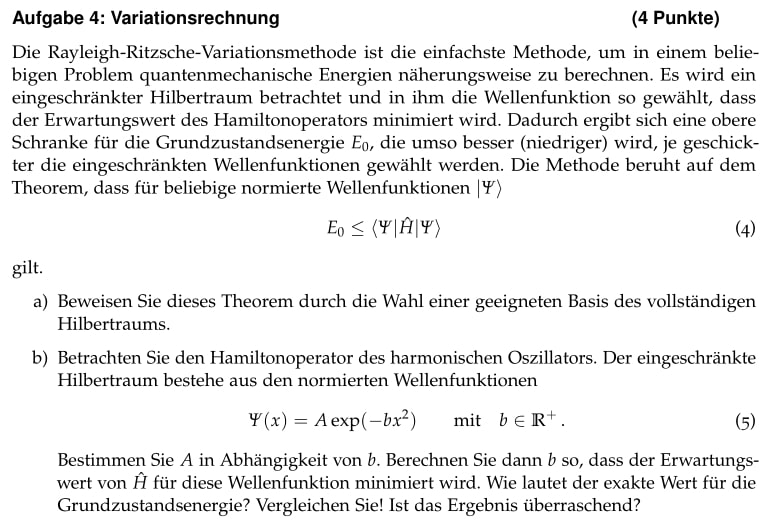
\includegraphics[width=\textwidth]{images/Aufgabe4a.jpg}
        \label{fig:5}
    \end{figure}

    \begin{figure}[H]
        \centering
        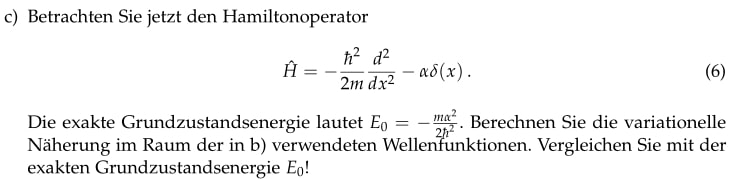
\includegraphics[width=\textwidth]{images/Aufgabe4b.jpg}
        \label{fig:6}
    \end{figure}

\subsection{a)}

    \flushleft{Als\;}\justifying geeignete Basis werden die Energieeigenzustände $\ket{\Psi} = \Psi_n \ket{n}$ verwendet.
    \begin{align*}
        \bra{\Psi} H \ket{\Psi} &= \sum_{n,m} \Psi_n^* \bra{n} H \ket{m} \Psi_m\\
        &= \sum_{n,m} \Psi_n^* \bra{n} E_m \ket{m} \Psi_m
        \intertext{
            \flushleft{Für\;}\justifying $E_m \leq E_0$ gilt:
        }
        &\leq \sum_{n,m} \Psi_n^* \bra{n} E_0 \ket{m} \Psi_m \qquad \text{mit}\; \braket{n}{m} = \delta_{nm} \;\text{und}\;n=m\\
        &\leq E_0 \sum_{n} \abs{\Psi_n}^2\\
        &\leq E_0 \underbrace{\braket{\Psi}{\Psi}}_{=1}\\
        \bra{\Psi} H \ket{\Psi} &\leq E_0
    \end{align*}

\subsection{b)}

    \begin{align*}
        \abs{\Psi(x)}^2 &= \int_{-\infty}^{\infty} \exp\left( -2bx^2 \right) \mathrm{d}x \stackrel{!}{=} 1\\
        \Leftrightarrow \abs{A}^2 \sqrt{\frac{\pi}{2b}} &= 1\\
        \abs{A}^2 &= \sqrt{\frac{2b}{\pi}}\\
        \\
        \hline\\
        \hat{H} &= \frac{\hat{p}^2}{2m} + \frac{m\omega^2}{2}\hat{x}^2\\
        \hat{p} \Psi &= -i\hbar \frac{\partial}{\partial x} \Psi\\
        \\
        \hline\\
        \langle H \rangle &= \int_{-\infty}^{\infty} \Psi^* \hat{H} \Psi \mathrm{d}x\\
        &= \int_{-\infty}^{\infty} A^* \exp\left( -bx^2 \right) \left( -\frac{\hbar^2}{2m} \frac{\partial^2}{\partial x^2} + \frac{m\omega^2}{2} \right) A \exp\left( -bx^2 \right) \mathrm{d}x\\
        &= \int_{-\infty}^{\infty} \abs{A}^2 \left( \frac{m\omega^2}{2} x^2 \exp\left( -2bx^2 \right) + \exp\left( -bx^2 \right) \frac{\hbar^2}{2m} \frac{\partial}{\partial x} \left( 2x \exp\left( -bx^2 \right) \right) \right) \mathrm{d}x\\
        &= \int_{-\infty}^{\infty} \sqrt{\frac{2b}{\pi}} \left( \frac{m\omega^2}{2} x^2 \exp\left( -2bx^2 \right) + \exp\left( -bx^2 \right) \frac{\hbar^2}{m} b \left( 1-2bx^2 \right) \exp\left( -bx^2 \right) \right) \mathrm{d}x\\
        &= \int_{-\infty}^{\infty} \sqrt{\frac{2b}{\pi}} \left( \frac{m\omega^2}{2} x^2 \exp\left( -2bx^2 \right) + \frac{\hbar^2}{m} b \left( 1-2bx^2 \right) \exp\left( -2bx^2 \right) \right) \mathrm{d}x\\
        &= \int_{-\infty}^{\infty} \sqrt{\frac{2b}{\pi}} \left( \left( \frac{m\omega^2}{2} - \frac{2\hbar^2 b^2}{m} \right) \exp\left( -2bx^2 \right) x^2 + \frac{\hbar^2 b}{m} \exp\left( -2bx^2 \right) \right) \mathrm{d}x\\
        &= \sqrt{\frac{2b}{\pi}} \frac{\hbar^2 b}{m} \sqrt{\frac{\pi}{2b}}\\
        &+ \left[ \sqrt{\frac{2b}{\pi}} \left( -\frac{1}{4b} \right) \left( \frac{m\omega^2}{2} - \frac{2\hbar^2 b^2}{m} \right) \exp\left( -2bx^2 \right) x \right]_{-\infty}^{\infty}\\
        &- \int_{-\infty}^{\infty} \sqrt{\frac{2b}{\pi}} \left( -\frac{1}{4b} \right) \left( \frac{m\omega^2}{2} - \frac{2\hbar^2 b^2}{m} \right) \exp\left( -2bx^2 \right) \mathrm{d}x\\
        &= \frac{\hbar^2 b}{m} + \frac{1}{4b} \left( \frac{m\omega^2}{2} - \frac{2\hbar^2 b^2}{m} \right)\\
        \Leftrightarrow\hat{H}(b) &= \frac{\hbar^2 b}{2m} + \frac{m\omega^2}{8b}\\
        \hat{H}'(b) &= \frac{\hbar^2}{2m} + \frac{m\omega^2}{8b^2}\\
        0 &= \frac{\hbar^2}{2m} + \frac{m\omega^2}{8b^2}\\
        \Leftrightarrow b &= \sqrt{ \frac{m^2 \omega^2}{4\hbar^2}} \qquad \text{$b$ kann hier nur $>0$ sein}\\
        &= \frac{m \omega}{2\hbar}\\
        \hat{H}_{\text{min}}(b) &= \frac{\hbar^2}{2m} \frac{m\omega}{2\hbar} + \frac{m\omega^2}{8} \frac{2\hbar}{m\omega}\\
        &= \frac{\hbar \omega}{4} + \frac{\hbar \omega}{4} = \frac{\hbar \omega}{2}
    \end{align*}

\subsection{c)}

\end{document}